\documentclass[aspectratio=169, 12pt]{beamer}

% --- Packages ---
\usepackage[utf8]{inputenc}
\usepackage[T1]{fontenc}
\usepackage{graphicx}
\usepackage{xcolor}
\usepackage{tcolorbox}
\usepackage{amsmath}
\usepackage{hyperref}
\usepackage{tikz}

% --- Theme & Styling ---
\usetheme{Madrid}
\usecolortheme{whale}

% Custom Colors (Matching the TrashUQ Brand)
\definecolor{TrashBlue}{HTML}{009688}
\definecolor{TrashDark}{HTML}{244c5a}
\definecolor{TrashAccent}{HTML}{3178c6}

\setbeamercolor{palette primary}{bg=TrashDark, fg=white}
\setbeamercolor{palette secondary}{bg=TrashBlue, fg=white}
\setbeamercolor{palette tertiary}{bg=TrashAccent, fg=white}
\setbeamercolor{titlelike}{parent=palette primary}
\setbeamercolor{structure}{fg=TrashBlue}

\setbeamertemplate{navigation symbols}{}
\setbeamertemplate{footline}[frame number]

% --- Title Information ---
\title[TrashUQ Presentation]{TrashUQ: Edge AI + Federated Learning}
\subtitle{Real-Time Intelligent Waste Management}
\author[Aleix, Bru, Pol]{
    Aleix Bertran Andreu \and Aleix Rosinach \\
    Bru \and Pol Llinàs
}
\date{May 2026}
\logo{
\includegraphics[height=0.8cm]{presentation_assets/cover.png}} % Placeholder for logo if needed

% --- Document ---
\begin{document}

% Slide 1: Title Slide with Background
{
\setbeamertemplate{background}{
\includegraphics[width=\paperwidth,height=\paperheight,keepaspectratio]{presentation_assets/cover.png}}
\begin{frame}[plain]
    % Empty frame to show background cover
\end{frame}
}

% Slide 2: Executive Summary
\begin{frame}{Executive Summary}
    \begin{columns}
        \begin{column}{0.6\textwidth}
            \begin{itemize}
                \item \textbf{TrashUQ} is an end-to-end platform for real-time trash classification monitoring.
                \item Integrates \textbf{Edge AI} on Arduino-class nodes with \textbf{Federated Learning} (FL).
                \item Combines MQTT telemetry, gRPC coordination, and a live Next.js dashboard.
                \item Successfully validated in a multi-node deployment with monotonic model versioning.
            \end{itemize}
        \end{column}
        \begin{column}{0.4\textwidth}
            \begin{tcolorbox}[colback=TrashBlue!10,colframe=TrashBlue,title=Key Features]
                \small
                \begin{itemize}
                    \item Real-time Observability
                    \item Scalable FL Coordinator
                    \item Concurrency Control
                    \item TFLite Material Classification
                \end{itemize}
            \end{tcolorbox}
        \end{column}
    \end{columns}
\end{frame}

% Slide 3: The Architecture (Visualized)
\begin{frame}{System Architecture}
    \begin{center}
        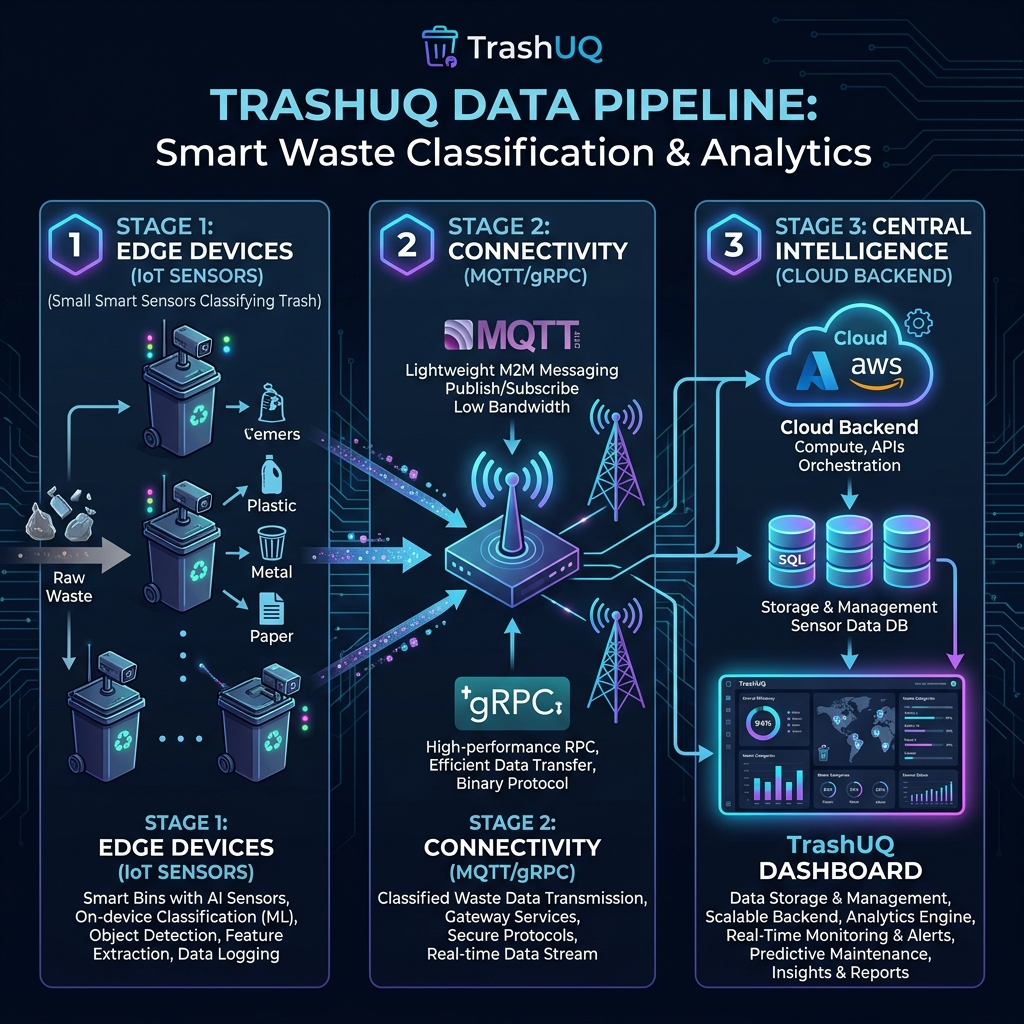
\includegraphics[width=0.85\textwidth]{presentation_assets/architecture.png}
    \end{center}
    \centering \small \textit{A three-stage pipeline: Edge Intelligence $\rightarrow$ Connectivity $\rightarrow$ Central Analysis}
\end{frame}

% Slide 4: Edge Intelligence & Classification
\begin{frame}{Edge Intelligence}
    \begin{columns}
        \begin{column}{0.5\textwidth}
            \textbf{On-Device Inference}
            \begin{itemize}
                \item Powered by \textbf{TensorFlow Lite (TFLite)}.
                \item Specialized for Arduino-class devices (UNO Q MPU).
                \item High-fidelity material classification.
            \end{itemize}
        \end{column}
        \begin{column}{0.5\textwidth}
            \textbf{Material Categories}
            \begin{itemize}
                \item \textcolor{TrashBlue}{Cardboard}
                \item \textcolor{TrashBlue}{Glass}
                \item \textcolor{TrashBlue}{Paper}
                \item \textcolor{TrashBlue}{Plastic}
            \end{itemize}
            \textit{Real-time performance: <100ms inference on edge hardware.}
        \end{column}
    \end{columns}
\end{frame}

% Slide 5: Telemetry & Connectivity
\begin{frame}{Connectivity & Telemetry}
    \begin{columns}
        \begin{column}{0.6\textwidth}
            \begin{itemize}
                \item \textbf{MQTT Protocol}: Lightweight pub/sub for real-time telemetry (status, metrics, events).
                \item \textbf{gRPC}: High-performance binary protocol for Federated Learning coordination.
                \item \textbf{Persistence}: PostgreSQL stores every message with full payload fidelity.
            \end{itemize}
        \end{column}
        \begin{column}{0.4\textwidth}
            \begin{tcolorbox}[colback=TrashDark!10,colframe=TrashDark,title=Data Integrity]
                \small
                \begin{itemize}
                    \item Monotonic versioning
                    \item Stale update rejection
                    \item 0\% dropped messages in validation
                \end{itemize}
            \end{tcolorbox}
        \end{column}
    \end{columns}
\end{frame}

% Slide 6: Federated Learning Coordinator
\begin{frame}{Federated Learning (FL) Lifecycle}
    \begin{center}
    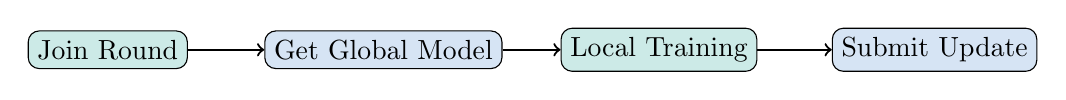
\begin{tikzpicture}[node distance=2cm, auto]
        \node (Join) [draw, rounded corners, fill=TrashBlue!20] {Join Round};
        \node (Get) [right of=Join, node distance=3.5cm, draw, rounded corners, fill=TrashAccent!20] {Get Global Model};
        \node (Train) [right of=Get, node distance=3.5cm, draw, rounded corners, fill=TrashBlue!20] {Local Training};
        \node (Submit) [right of=Train, node distance=3.5cm, draw, rounded corners, fill=TrashAccent!20] {Submit Update};
        \draw [->, thick] (Join) -- (Get);
        \draw [->, thick] (Get) -- (Train);
        \draw [->, thick] (Train) -- (Submit);
    \end{tikzpicture}
    \end{center}
    \vspace{0.5cm}
    \begin{itemize}
        \item \textbf{FedAvg Aggregation}: Weighted averaging based on sample count.
        \item \textbf{Coordination}: Handled via gRPC \texttt{SubmitUpdate} workflows.
        \item \textbf{Stability}: Proven convergence under Non-IID data partitions.
    \end{itemize}
\end{frame}

% Slide 7: Live Dashboard
\begin{frame}{Live Monitoring Dashboard}
    \begin{center}
        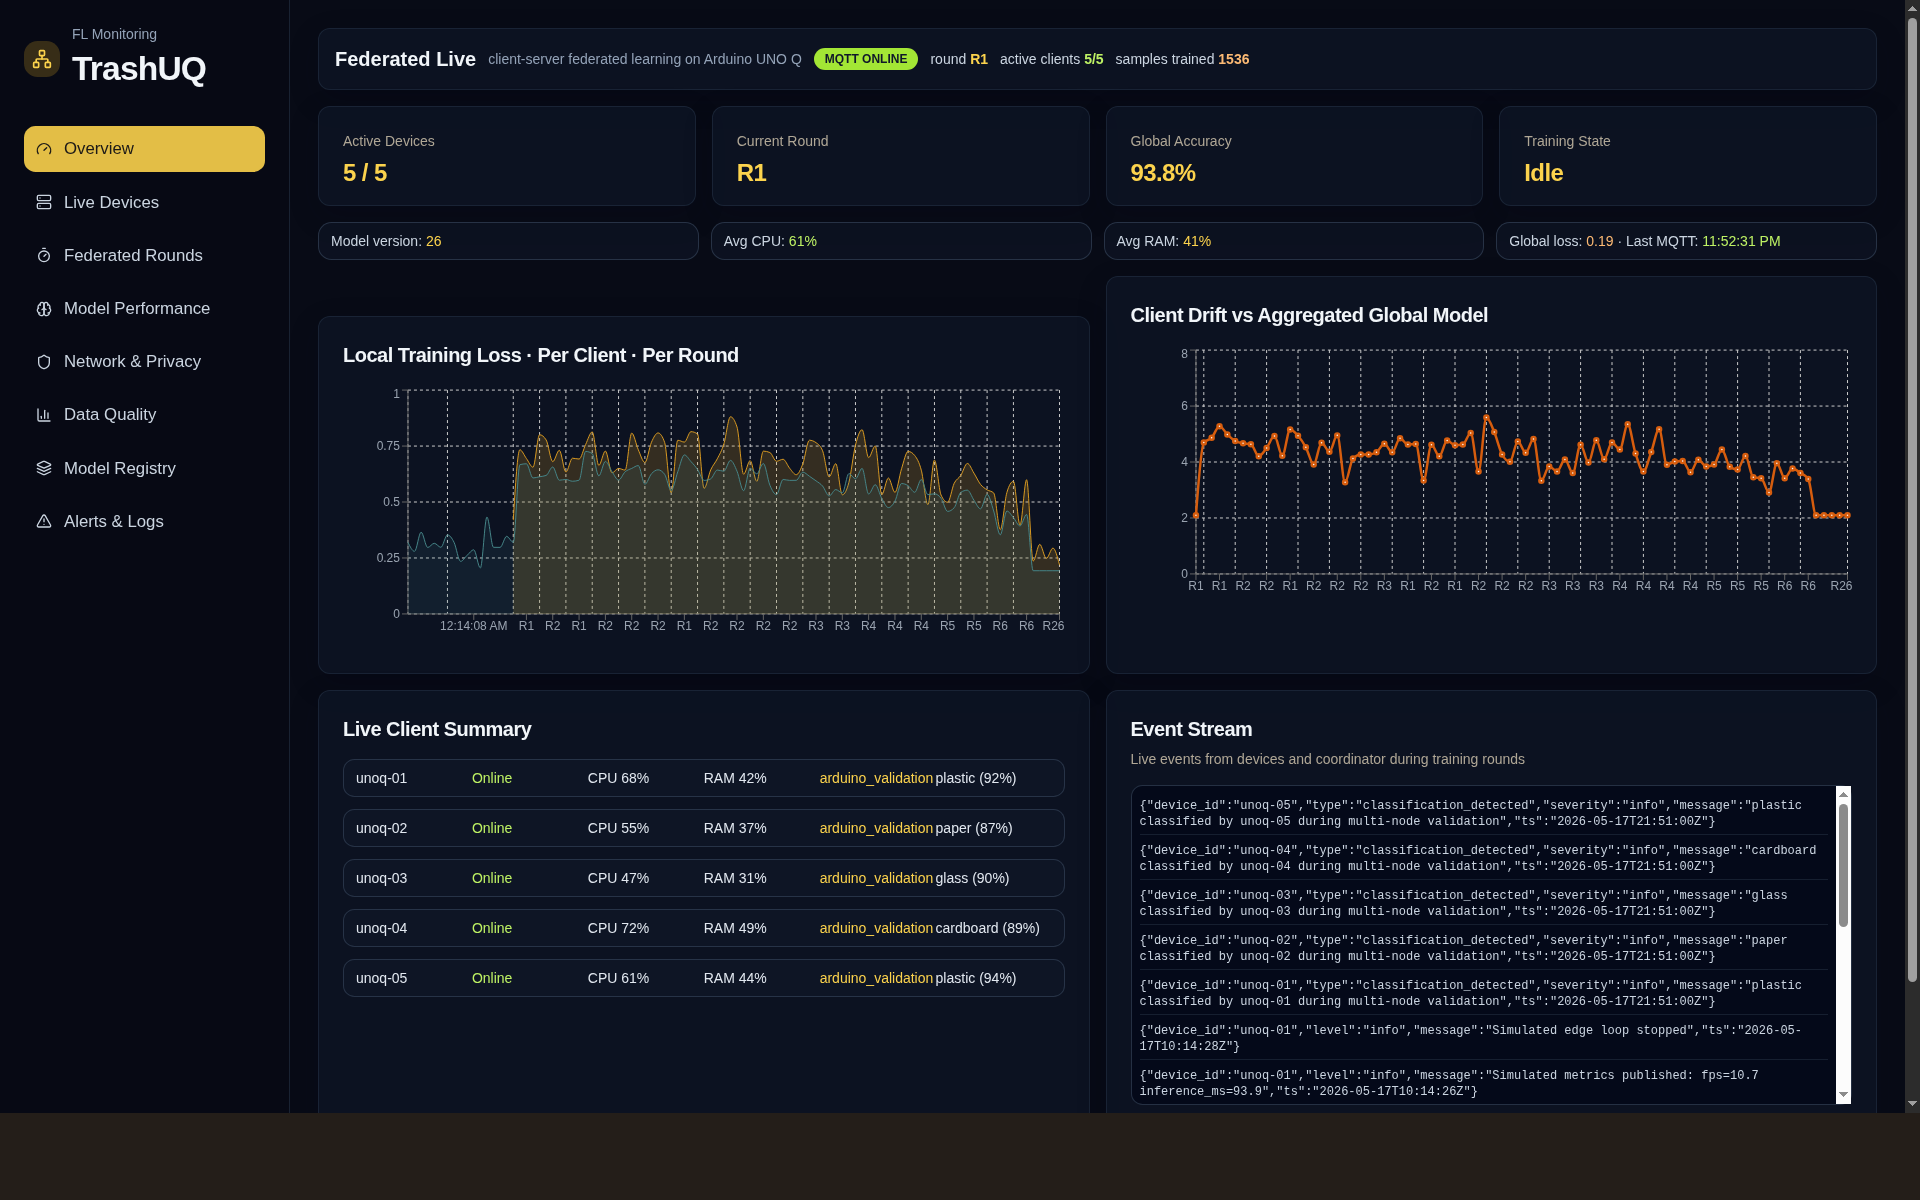
\includegraphics[width=0.85\textwidth]{presentation_assets/dashboard.png}
    \end{center}
    \centering \small \textit{Next.js Dashboard: Real-time charts, device status, and FL progress streams.}
\end{frame}

% Slide 8: Validation Results (Part A)
\begin{frame}{Validation Highlights (Part A)}
    \begin{columns}
        \begin{column}{0.5\textwidth}
            \begin{itemize}
                \item \textbf{Deployment}: 2 Arduino nodes on \texttt{bepes-server}.
                \item \textbf{Activity}: 282 MQTT messages persisted.
                \item \textbf{Progress}: 26 FL rounds completed.
                \item \textbf{Success}: Model version advanced from 0 to 26.
            \end{itemize}
        \end{column}
        \begin{column}{0.5\textwidth}
            \begin{table}
                \centering
                \begin{tabular}{|l|r|}
                \hline
                \textbf{Metric} & \textbf{Value} \\ \hline
                Aggregation Success & 83.3\% \\ \hline
                Invalid Payload Rate & 0\% \\ \hline
                Dashboard Lag & < 1s \\ \hline
                Median Latency & $\sim$25ms \\ \hline
                \end{tabular}
            \end{table}
        \end{column}
    \end{columns}
\end{frame}

% Slide 9: Scalability Study (Part B)
\begin{frame}{Scalability & Performance (Part B)}
    \begin{itemize}
        \item \textbf{Experiment}: Evaluated scaling from 2 to 20 clients.
        \item \textbf{Data}: Dirichlet Non-IID partitioning ($\alpha=0.3$).
        \item \textbf{Accuracy}: Maintained \textbf{93-94\% accuracy} across all scales.
        \item \textbf{Efficiency}: Communication cost scaled linearly with client count.
    \end{itemize}
    \begin{center}
    \begin{tcolorbox}[colback=TrashBlue!5,colframe=TrashBlue, width=0.7\textwidth]
        \centering \small \textbf{Result:} Stable convergence even under highly heterogeneous data.
    \end{tcolorbox}
    \end{center}
\end{frame}

% Slide 10: Conclusion & Roadmap
\begin{frame}{Conclusion \& Future Roadmap}
    \begin{columns}
        \begin{column}{0.5\textwidth}
            \textbf{Achievements}
            \begin{itemize}
                \item Proven edge-to-cloud FL pipeline.
                \item Robust concurrency and persistence.
                \item Deployed hardware validation.
            \end{itemize}
        \end{column}
        \begin{column}{0.5\textwidth}
            \textbf{Future Directions}
            \begin{itemize}
                \item Production authentication & IAM.
                \item Fleet management for 100+ nodes.
                \item Advanced FL analytics & Differential Privacy.
            \end{itemize}
        \end{column}
    \end{columns}
\end{frame}

% Slide 11: Team
\begin{frame}{The TrashUQ Team}
    \begin{center}
        \Huge \textbf{Thank You!} \\
        \vspace{1cm}
        \large
        Aleix Bertran Andreu \quad Aleix Rosinach \\
        Bru \quad Pol Llinàs
    \end{center}
\end{frame}

\end{document}
